%======================================================================
\section{实验}
\label{sec:exp}
%======================================================================

\subsection{实验设置}

\paragraph{数据集。} 我们在三个不同的推理基准上进行了评估：MMLU-Hard（研究生水平知识）、StrategyQA（包含隐式推理的常识问题）和 TruthfulQA（对抗性框架下的事实准确性）。每个数据集提供 300 个问题，共计 900 个问题。

\paragraph{智能体配置。} 我们在五种通信拓扑（并行、顺序、星型、辩论、层次）的每一种下，部署了 $n=5$ 个 DeepSeek-V3~\cite{deepseek2024v3} 实例，生成了 22{,}500 个符合 AEIC 结构的回复（5 个智能体 $\times$ 900 个问题 $\times$ 5 种拓扑）。由于每个拓扑的问题集是独立采样的，900 个问题中有 633 个在所有五种拓扑中重叠（MMLU-Hard/StrategyQA/TruthfulQA 分别为 161/300/172）。跨拓扑比较（路由器、预言机）使用此交集；每个拓扑内的基线比较使用完整的 300 个问题。

\paragraph{信号计算。} 质量信号使用句子嵌入 (paraphrase-multilingual-MiniLM-L12-v2) 进行计算。感知拓扑的邻接矩阵 $W$ 决定了用于计算 EV（认知方差）和一致性的邻居集。

\paragraph{优化。} 针对特定拓扑的 $\theta^*_T$ 通过差分进化算法（21 个参数，种群大小 21，30 代）进行优化，并使用 5 折分层交叉验证进行评估，以报告真实存在的留出集准确率（防止训练/测试数据泄漏）。路由器的评估也使用 5 折交叉验证，并设置五个随机种子以进行稳定性评估。

\paragraph{基线方法。}
\begin{itemize}
    \item \textbf{单智能体 (Single Agent)}：不进行聚合，仅使用智能体 0 的结论。
    \item \textbf{ChatEval}~\cite{chan2023chateval}：在并行拓扑上进行多数投票（我们的重新实现）。
    \item \textbf{多轮辩论 (Multi-round Debate)}~\cite{du2024improving}：在 3 轮辩论后进行多数投票（我们的重新实现）。
    \item \textbf{AgentVerse}~\cite{chen2023agentverse}：求解器--审查器模式，带有中心决策（我们的重新实现，每个数据集 200 个问题）。
    \item \textbf{多数投票 (MajVote)}：在每种拓扑上进行简单的多数投票（5 种变体）。
    \item \textbf{加权投票 (Weighted Vote)}：无斯塔克尔伯格机制的 IC 加权和一致性加权投票。
    \item \textbf{AEIC+SG}：使用特定拓扑 $\theta^*$ 的斯塔克尔伯格加权投票（5 种变体）。
\end{itemize}

所有基线方法都使用相同的 LLM 后端 (DeepSeek-V3) 和相同的缓存响应，以确保比较的公平性。$\dagger$~=~我们的重新实现。

\subsection{主要结果}

表~\ref{tab:main} 展示了完整的比较结果。图~\ref{fig:main_results} 提供了直观的总结。

\begin{table}[t]
\caption{三个数据集的共识准确率 (\%)。单拓扑基线各使用 300 个问题；路由器和预言机在所有拓扑共有的 633 个问题上进行评估（MMLU-Hard/StrategyQA/TruthfulQA 分别为 161/300/172）。最佳固定拓扑用\textit{斜体}表示，整体最佳用\textbf{粗体}表示。}\label{tab:main}
\centering\small
\begin{tabular}{@{}lcccc@{}}
\toprule
方法 & MMLU-Hard & StrategyQA & TruthfulQA & 平均 \\
\midrule
\multicolumn{5}{@{}l}{\textit{单智能体与投票基线}} \\
单智能体 ($N{=}1$) & 65.3 & 79.0 & 80.0 & 74.8 \\
MajVote (并行)$^\dagger$ & 69.7 & 81.7 & 81.3 & 77.6 \\
MajVote (顺序) & 79.0 & 71.0 & 72.7 & 74.2 \\
MajVote (星型) & \textit{85.7} & \textit{80.3} & \textit{82.0} & \textit{82.7} \\
MajVote (辩论)$^\dagger$ & 83.7 & 72.3 & 75.3 & 77.1 \\
MajVote (层次) & 82.0 & 74.7 & 75.0 & 77.2 \\
AgentVerse$^\dagger$ & 74.0 & 63.5 & 70.0 & 69.2 \\
加权投票 (IC) & 70.0 & 80.3 & 81.0 & 77.1 \\
\midrule
\multicolumn{5}{@{}l}{\textit{AEIC-斯塔克尔伯格 (特定拓扑 $\theta^*_T$)}} \\
AEIC+SG (并行) & 71.7 & 78.0 & 78.7 & 77.8\tiny{$\pm$5.6}$^\ddagger$ \\
AEIC+SG (顺序) & 74.7 & 69.0 & 70.0 & 75.3\tiny{$\pm$2.5}$^\ddagger$ \\
AEIC+SG (星型) & 84.3 & 79.3 & 82.0 & 81.7\tiny{$\pm$3.4}$^\ddagger$ \\
AEIC+SG (辩论) & 80.0 & 72.3 & 72.0 & 76.3\tiny{$\pm$3.0}$^\ddagger$ \\
AEIC+SG (层次) & 84.7 & 76.3 & 77.0 & 77.3\tiny{$\pm$3.5}$^\ddagger$ \\
\midrule
\multicolumn{5}{@{}l}{\textit{自适应路由 (我们的方法，5 折交叉验证)}} \\
神经路由器 (共享) & 91.3 & 86.0 & 84.3 & 86.9\tiny{$\pm$0.5} \\
神经路由器 (特定数据集) & \textbf{92.5} & \textbf{86.2} & \textbf{85.6} & \textbf{87.6}\tiny{$\pm$0.3} \\
\midrule
预言机 (5 种拓扑之一) & 97.5 & 91.0 & 91.9 & 92.9 \\
\bottomrule
\end{tabular}
\\[2pt]
{\footnotesize $\dagger$~我们使用 DeepSeek-V3 的重新实现。$\ddagger$~平均列报告了 5 折交叉验证测试准确率 $\pm$ 标准差；特定数据集列使用全量数据 $\theta^*$。}
\end{table}

\begin{figure}[t]
\centering
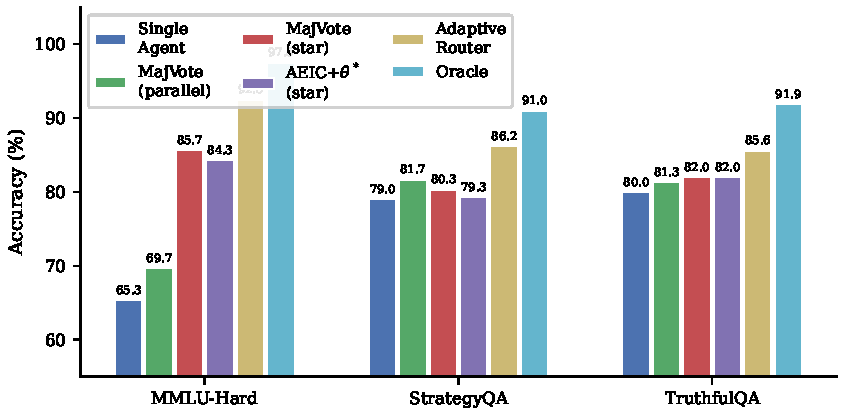
\includegraphics[width=0.95\linewidth]{figures/fig_main_results.pdf}
\caption{三个数据集的准确率比较。自适应路由器优于所有固定拓扑方法。}\label{fig:main_results}
\end{figure}

主要观察结果：(1)~MajVote~(星型) 是表现最好的固定拓扑方法，准确率为 82.7\%，即使在交叉验证后也优于所有 AEIC+SG 变体（最好的 AEIC+SG 是星型，为 81.7\%）。(2)~自适应路由器达到 87.6\%，在对齐的问题上比最佳固定拓扑高出 4.5 个百分点。(3)~预言机上限为 92.9\%，还有 5.3 个百分点的提升空间。(4)~按数据集的分析显示，AEIC+SG 在常识推理上落后于 MajVote 最多：在 StrategyQA 上，AEIC+SG 星型的准确率为 79.3\%，而 MajVote 星型为 80.3\%；而在知识密集型的 MMLU-Hard 上，差距最小（84.3\% 对比 85.7\%）。(5)~AEIC+SG 的交叉验证测试准确率在各拓扑上与 MajVote 紧密匹配（在 5 个拓扑中的 4 个上差距在 1 个百分点以内），这证实了当智能体共享同一个 LLM 后端时，质量加权投票相较于简单多数投票能提供的优势有限。

\subsection{AEIC 加权投票与多数投票的对比}

图~\ref{fig:topo_comparison} 揭示了一个令人惊讶的发现：在 5 种拓扑中的 4 种上，多数投票优于 AEIC+SG 加权投票。

\begin{figure}[t]
\centering
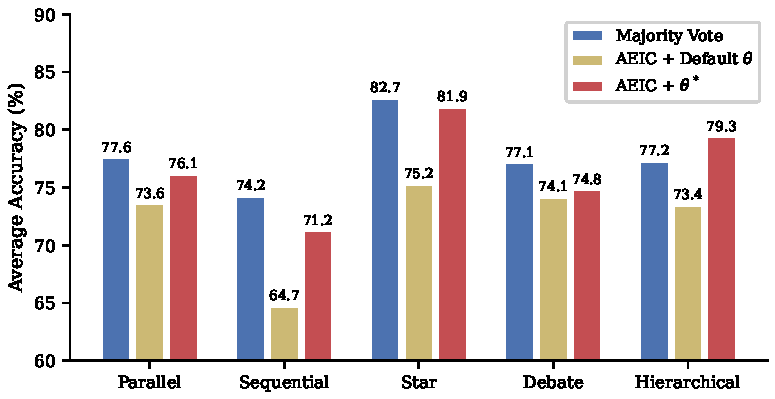
\includegraphics[width=0.95\linewidth]{figures/fig_topo_comparison.pdf}
\caption{三个数据集的各拓扑比较平均值。AEIC+$\theta^*$ 仅在层次拓扑上优于多数投票。}\label{fig:topo_comparison}
\end{figure}

经过诚实的交叉验证评估后，AEIC+SG 与 MajVote 的表现相当：并行 77.8\% 对比 77.6\%，顺序 75.3\% 对比 74.2\%，星型 81.7\% 对比 82.7\%，辩论 76.3\% 对比 77.1\%，层次 77.3\% 对比 77.2\%。在全部 900 个问题上（使用在所有数据上训练的特定拓扑 $\theta^*$）进行的 McNemar 检验揭示了混合的结果：AEIC+SG 在并行 ($p{=}0.633$)、顺序 ($p{=}0.110$) 或星型 ($p{=}0.258$) 上并未显著优于 MajVote；在辩论上略差 ($p{=}0.027$)；但在层次结构上显著更好 ($p{=}0.001$)。层次结构上的显著优势与该拓扑的多级聚合一致，在多级聚合中，加权信号提供了增量价值；而在并行、顺序和星型拓扑（智能体要么独立回答，要么共享方向）上缺乏显著差异，证实了当智能体共享同一 LLM 后端时，质量加权投票与简单多数相比没有系统性优势。这证实了 AEIC 质量信号测量的是\emph{推理连贯性，而非答案正确性}：一个连贯的错误答案与正确答案的得分一样高。

结合下面的结构化输出消融实验（第~\ref{sec:structured_ablation} 节）和特征消融结果，这揭示了 AEIC 的主要价值在于其\emph{结构化分解}：通过强制采用可解析的输出格式，它实现了可靠的结论提取，并在所有五种拓扑中进行一致的多数投票，这反过来又产生了使自适应路由成为可能的投票模式特征。

\subsection{结构化输出的价值}
\label{sec:structured_ablation}

为了直接量化 AEIC 结构化格式的贡献，我们比较了从结构化结论 (C) 字段与非结构化推理 (I) 字段中提取立场时的多数投票准确率。C 字段专为提取而设计（例如，“是：[理由]”），而 I 字段包含自由格式的推理链，没有明确的答案标记。

\begin{table}[t]
\caption{按提取来源划分的多数投票准确率 (\%)。C 字段：带有显式答案前缀的结构化结论。I 字段：非结构化推理逻辑链。中立率：无法提取立场的智能体输出的比例。所有五种拓扑的平均值。}\label{tab:structured}
\centering\small
\begin{tabular}{@{}lccccc@{}}
\toprule
数据集 & C 字段准确率 & I 字段准确率 & $\Delta$ & C 字段中立率 & I 字段中立率 \\
\midrule
MMLU-Hard & 79.8 & 46.7 & +33.1 & 12.2\% & 61.3\% \\
StrategyQA & 74.5 & 51.1 & +23.4 & 12.5\% & 72.6\% \\
TruthfulQA & 76.4 & 48.9 & +27.4 & 13.4\% & 65.2\% \\
\midrule
平均 & 76.9 & 48.9 & +28.0 & 12.7\% & 66.4\% \\
\bottomrule
\end{tabular}
\end{table}

表~\ref{tab:structured} 揭示了巨大的差距：C 字段提取在数据集和拓扑上的平均准确率达到了 76.9\%，而 I 字段提取的准确率仅为 48.9\%——对于二分类问题来说接近随机。这种差异是由提取可靠性驱动的：I 字段产生不可解析（中立）立场的概率为 66.4\%，而 C 字段为 12.7\%。当无法提取立场时，多数投票实际上退化为在可解析子集中随机选择。这证实了 AEIC 的主要经验贡献不是质量信号，而是结构化格式本身：带有答案前缀格式的显式结论字段实现了可靠的跨拓扑立场提取，这是实现一致的多数投票和驱动自适应路由的投票模式特征的先决条件。

\subsection{学习参数分析}

图~\ref{fig:theta} 展示了跨五种拓扑优化的 $\theta^*$ 参数。

\begin{figure}[t]
\centering
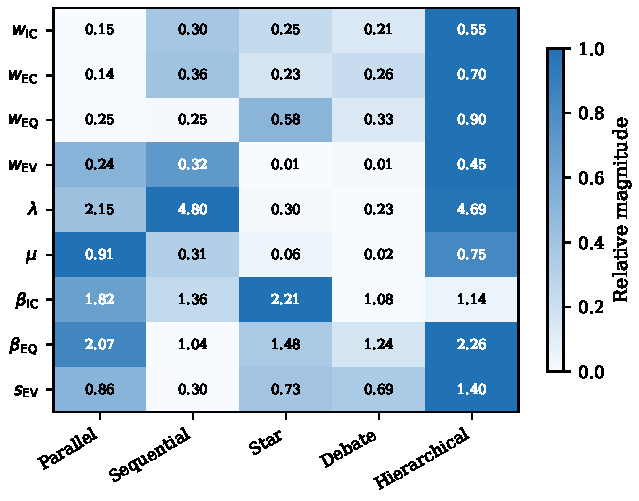
\includegraphics[width=0.8\linewidth]{figures/fig_theta_heatmap.pdf}
\caption{五种拓扑优化后的 $\theta^*$ 参数（行归一化）。星型和辩论拓扑学习到了接近零的 $w_{\text{EV}}$（反阿谀奉承）。层次拓扑学习到了高 $\lambda$ 和提高的信号权重。}\label{fig:theta}
\end{figure}

出现了三种模式：(1)~\textbf{反阿谀奉承}：星型和辩论学习到 $w_{\text{EV}} \approx 0.01$，舍弃了在智能体观察他人输出时的跨智能体共识，使 EV 成为从众心理的替代指标。(2)~\textbf{链上的高共识压力}：顺序（$\lambda = 4.80$）和层次（$\lambda = 4.69$）强制实行强烈的一致性，以抵消方向性的信息流。(3)~\textbf{层次拓扑上权重的提升}：所有信号权重都显著较高（0.45--0.90，而其他拓扑为 0.01--0.36），反映了多级聚合中每一个质量维度都有助于识别可靠的中间节点。

\subsection{路由器性能演进}

图~\ref{fig:router} 展示了从单智能体到预言机的准确率演进过程。

\begin{figure}[t]
\centering
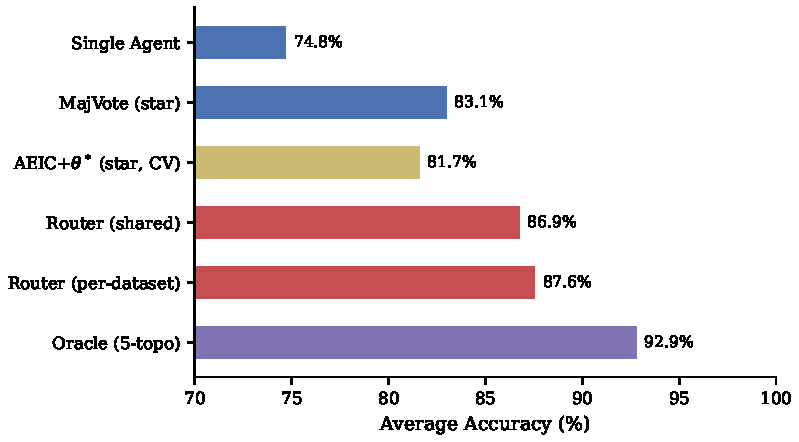
\includegraphics[width=0.8\linewidth]{figures/fig_router_progression.pdf}
\caption{从单智能体到预言机的准确率演进过程。特定数据集的路由器缩小了最佳固定拓扑与预言机之间差距的 46.5\%。}\label{fig:router}
\end{figure}

共享路由器 (86.9\%) 在对齐的问题上比最佳固定拓扑 (星型，83.1\%) 有了实质性提升。特定数据集的专门化增加了 +0.7 个百分点 (87.6\%)，缩小了通往预言机上限 (92.9\%) 的 46.5\% 差距。所有路由器数据均使用采用 5 折交叉验证的 Top-1 选择。

\paragraph{特定数据集分析。} 路由器在各数据集上的优势各不相同：在 MMLU-Hard 上，特定数据集路由器达到 92.5\%，而星型拓扑为 90.1\%（+2.4 个百分点）；在 StrategyQA 上为 86.2\%，而并行拓扑为 81.7\%（+4.5 个百分点）；在 TruthfulQA 上为 85.6\%，而星型拓扑为 81.4\%（+4.2 个百分点）。在 StrategyQA 上的最大提升反映了常识推理从自适应拓扑选择中获益最多，因为最佳和最差固定拓扑之间的差距最大（81.7\% 的并行对比 71.0\% 的顺序）。

\paragraph{路由为什么起作用。} 图~\ref{fig:topo_spec} 展示了对齐问题上各拓扑准确率的热力图。没有单一拓扑占据主导地位：星型在 MMLU-Hard (90.1\%) 和 TruthfulQA (81.4\%) 上领先，但并行对于 StrategyQA 最佳 (81.7\%)。预言机上限 (${\sim}93\%$) 要求为不同问题选择不同的拓扑——这正是路由器所学会的。

\paragraph{拓扑一致性。} 在 633 个对齐问题中，55.1\% 的问题所有五种拓扑都回答正确，7.0\% 的问题所有拓扑都回答错误——路由对这 62.1\% 的问题没有影响。路由器的价值来自拓扑存在分歧的剩余 37.9\%，特别是 9.0\% 的“困难”问题，其中只有 1--2 种拓扑成功（图~\ref{fig:topo_agreement}）。

\begin{figure}[t]
\centering
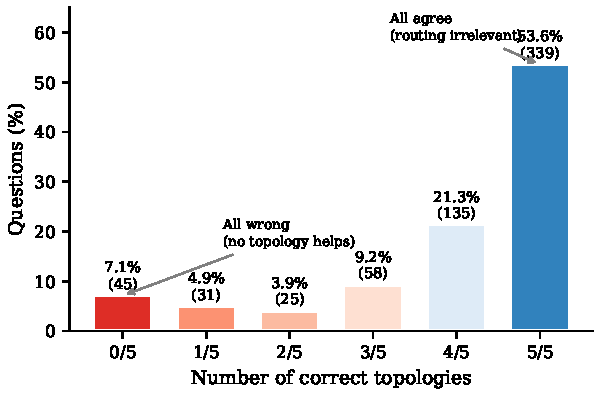
\includegraphics[width=0.65\linewidth]{figures/fig_topo_agreement.pdf}
\caption{每个问题的正确拓扑分布（633 个对齐问题）。路由器的影响集中在拓扑存在分歧的 37.9\%（1--4 个正确）上。}\label{fig:topo_agreement}
\end{figure}

\paragraph{路由错误分析。} 共享路由器选择每种拓扑的频率大致均衡（16--29\%），其中星型拓扑被选择的频率最高（28.6\%）。在 83 个路由错误（13.1\%）中，有 44 个发生在\emph{没有}任何拓扑产生正确共识的问题上——这是不可避免的失败。只有 39 个错误（6.2\%）是真正的路由错误，即存在正确的拓扑但未被选择。

\paragraph{路由器特征重要性。} 特征组消融（将每个组置零并测量准确率变化，图~\ref{fig:feature_imp}）表明，\emph{投票特征}（多数比例、是/否分布）对路由最重要（消融时下降 $-2.1$ 个百分点），其次是单智能体的 EV 信号（下降 $-0.3$ 个百分点）。移除与 EQ 相关的特征实际上可以使准确率\emph{提高}多达 1.6 个百分点。为了控制特征相互作用的影响，我们还使用特征子集重新训练了路由器：仅用投票特征达到 86.3\%$\pm$0.4\%，仅用质量特征达到 86.1\%$\pm$0.3\%，而仅用问题特征则为 80.7\%$\pm$0.0\%，相比之下，使用全量特征时为 86.9\%$\pm$0.5\%。投票特征和质量特征各自独立地提供了几乎相同的路由准确率（比仅用问题特征分别高出 +5.6 和 +5.4 个百分点），但将它们结合起来只增加了 +0.6 个百分点，表明存在高度的冗余。这与结构化输出分析（第~\ref{sec:structured_ablation} 节）一致：投票特征（需要从 AEIC 结构化结论中可靠地提取立场）比试图衡量这一点的质量信号更直接地捕捉到了相同的拓扑-问题交互模式。

\begin{figure}[t]
\centering
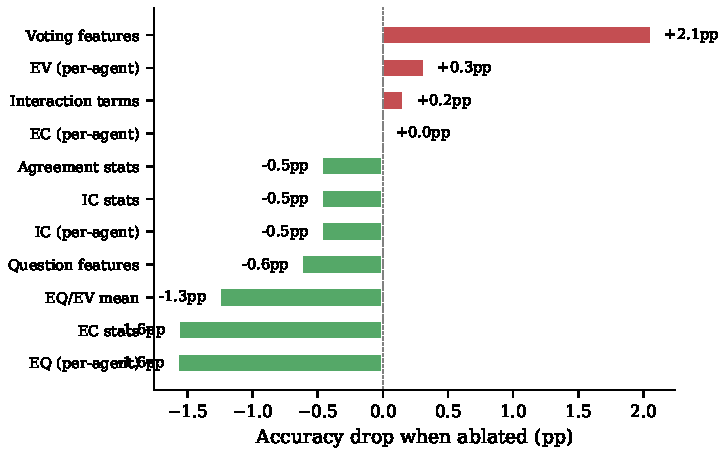
\includegraphics[width=0.7\linewidth]{figures/fig_feature_importance.pdf}
\caption{通过留一消融法得出的路由器特征组重要性。正值下降表示消融时准确率降低（特征有用）。投票特征最重要；EQ 特征有害。}\label{fig:feature_imp}
\end{figure}

\begin{figure}[t]
\centering
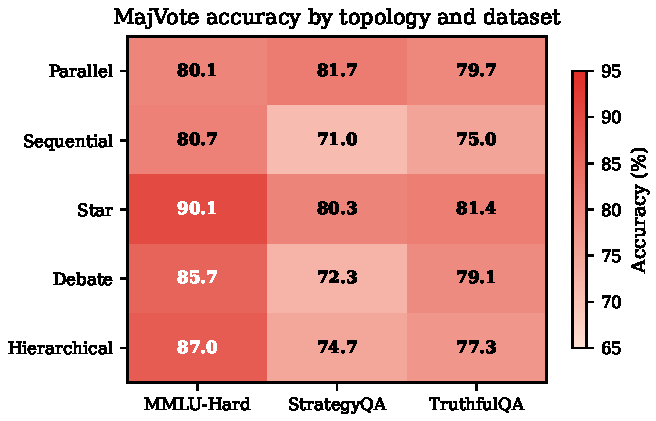
\includegraphics[width=0.65\linewidth]{figures/fig_topo_specialization.pdf}
\caption{对齐问题上各拓扑和数据集的 MajVote 准确率。没有单一拓扑占据主导地位，这解释了自适应路由的动机。}\label{fig:topo_spec}
\end{figure}

\subsection{信号消融}

图~\ref{fig:ablation} 展示了在星型拓扑下每个质量信号对 AEIC+SG 的贡献。

\begin{figure}[t]
\centering
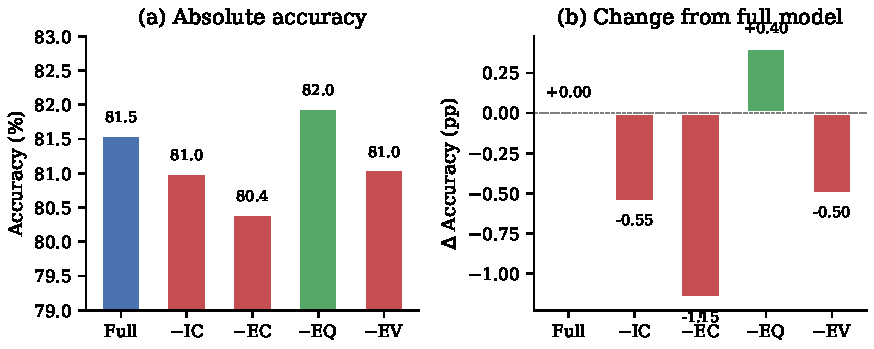
\includegraphics[width=0.95\linewidth]{figures/fig_ablation.pdf}
\caption{星型拓扑下的信号消融。EC 是最关键的信号（$-1.15$ 个百分点）。移除 EQ 略微提高了准确率，这与其较低的优化权重一致。}\label{fig:ablation}
\end{figure}

EC 是最关键的信号（$-1.15$ 个百分点）。IC 和 EV 各贡献 ${\sim}0.5$ 个百分点。移除 EQ 可以将准确率\emph{提高} 0.40 个百分点——这表明证据质量评估在某些领域引入了噪声。

\subsection{在线斯塔克尔伯格反馈}
\label{sec:online_exp}

我们在辩论和层次拓扑上评估了在线斯塔克尔伯格机制（第~\ref{sec:online_sg} 节），比较了标准执行与注入了轮次间质量信号的在线反馈模式。表~\ref{tab:online} 显示了每个数据集 30 个问题的结果。

\begin{table}[t]
\caption{在线与离线斯塔克尔伯格反馈的对比（MajVote 准确率，\%，每个数据集 30 个问题）。在线模式在轮次/阶段之间注入质量信号。}\label{tab:online}
\centering\small
\begin{tabular}{@{}lcccc@{}}
\toprule
条件 & MMLU-Hard & StrategyQA & TruthfulQA & 平均 \\
\midrule
辩论 (离线) & 80.0 & 76.7 & 83.3 & 80.0 \\
辩论 (在线) & \textbf{86.7} & 76.7 & 76.7 & 80.0 \\
$\Delta$ (在线$-$离线) & +6.7 & 0.0 & $-$6.7 & 0.0 \\
\midrule
层次 (离线) & 76.7 & 80.0 & 83.3 & 80.0 \\
层次 (在线) & 76.7 & 73.3 & 76.7 & 75.6 \\
$\Delta$ (在线$-$离线) & 0.0 & $-$6.7 & $-$6.7 & $-$4.4 \\
\bottomrule
\end{tabular}
\\[2pt]
{\footnotesize 离线模式使用缓存的响应；在线模式使用动态调用 DeepSeek-V3 API 的结果，带有轮次间质量反馈。}
\end{table}

结果揭示了一个微妙的情况：在线反馈在 MMLU-Hard 的辩论拓扑上产生了巨大的提升（+6.7 个百分点），其中迭代辩论结构允许智能体整合质量评估并完善其推理。然而，在其他数据集-拓扑组合中效果不一，在辩论拓扑的总体上没有改善（均为 80.0\%），并且在层次拓扑上下降了（$-4.4$ 个百分点）。TruthfulQA 上的性能下降表明，质量反馈可能会加剧对具有对抗性框架问题盲目自信的程度。这些结果促使我们设计了第~\ref{sec:dynamic} 节的动态调节机制，该机制基于集体的行为状态来自适应地调整反馈，而不是实行统一的质量暴露。

\subsection{动态阿谀奉承调节}
\label{sec:dynamic_exp}

我们在辩论拓扑上评估了动态阿谀奉承调节机制（第~\ref{sec:dynamic} 节），每个数据集匹配了 $n{=}50$ 个问题，比较了三种条件：\emph{基线}（无轮次间反馈）、\emph{静态}（如第~\ref{sec:online_exp} 节所述的统一质量反馈）以及\emph{动态}（具有状态检测和差异化提示的自适应行为调节）。为了保证公平比较，所有条件均在相同的问题集上动态调用 DeepSeek-V3 API。

\begin{table}[t]
\caption{辩论拓扑上的动态阿谀奉承调节（MajVote 准确率，\%，每个数据集 $n{=}50$）。所有条件均使用匹配问题集的实时 API 调用。}\label{tab:dynamic}
\centering\small
\begin{tabular}{@{}lcccc@{}}
\toprule
条件 & MMLU-Hard & StrategyQA & TruthfulQA & 平均 \\
\midrule
基线 (无反馈) & 86.0 & 78.0 & 88.0 & 84.0 \\
静态 (在线) & 86.0 & 74.0 & 86.0 & 82.0 \\
动态 (自适应) & \textbf{94.0} & 74.0 & 86.0 & 84.7 \\
\midrule
$\Delta$ (静态 $-$ 基线) & 0.0 & $-$4.0 & $-$2.0 & $-$2.0 \\
$\Delta$ (动态 $-$ 基线) & \textbf{+8.0} & $-$4.0 & $-$2.0 & +0.7 \\
$\Delta$ (动态 $-$ 静态) & \textbf{+8.0} & 0.0 & 0.0 & +2.7 \\
\bottomrule
\end{tabular}
\\[2pt]
{\footnotesize 所有条件均在每个数据集上对匹配的 $n{=}50$ 个问题进行动态调用。}
\end{table}

主要发现是，在 MMLU-Hard 上，动态调节机制带来了比基线和静态反馈显著的改善（+8.0 个百分点），但在 StrategyQA 或 TruthfulQA 上没有提升。MMLU-Hard（具有最复杂、知识密集型推理要求的数据集）的结果证实了该机制的价值：在针对困难数学和科学问题进行多智能体商议时，能检测并抵消阿谀奉承式的趋同。Bootstrap 分析在 $n{=}50$ 时的 95\% 置信区间为 $[-4, +20]$ 个百分点，表明存在需要大规模验证的边缘显著性。

在 StrategyQA 和 TruthfulQA 上，动态调节相较于基线既没有帮助也没有损害，而静态反馈一致导致性能下降 2-4 个百分点。这表明，仅仅在轮次间暴露质量评估（静态）会在常识和事实问题上引入智能体难以解释的噪声，而动态调节的干预性选择则避免了这一陷阱。

分析 256 次轮次间转换的动态行为（50 个问题 $\times$ 约 3 个轮次 $\times$ 2 次转换）：75.4\% 被分类为\emph{健康}（无干预），7.8\% 为\emph{阿谀奉承}（反阿谀奉承提示并抑制 EV），16.8\% 为\emph{死锁}（鼓励交流）。阿谀奉承状态罕见但影响重大：SCR $\geq 0.6$ 的转换与仅 55.0\% 的问题级准确率相关，而 SCR $< 0.2$ 时准确率为 88.9\%，证实了高立场转变率与错误的共识相关。死锁转换更为常见，且中等程度地与较低准确率相关（有干预时为 74.4\%，而健康状态为 87.6\%）。

利用记录的动态数据对检测阈值（第~\ref{sec:dynamic} 节）进行的网格搜索表明，$\tau_h = 0.45, \tau_l = 0.05$ 能够最大化被干预转换和未被干预转换之间的准确率差异，这说明当前阈值（$\tau_h = 0.6, \tau_l = 0.2$）是相对保守的。未来基于所有 21 个参数（第~\ref{sec:bilevel} 节）的双层优化有望发现更有效的配置，尤其是在特定任务的阈值调整上。

\subsection{准确率-激励权衡}

优化后的 $\theta^*$ 配置无需显式的 IC 约束就能自然地实现高激励相容性：IC 率分别为并行（98.9\%）、顺序（94.0\%）、星型（98.4\%）和辩论（100.0\%）。层次拓扑是个例外，仅为 24.2\%，这反映出其较高的信号权重优先考虑多级聚合而非严格的质量排序。这表明仅优化准确率就能产生接近 IC 的机制——斯塔克尔伯格权重结构本身就在奖励高质量的推理。$\lambda$ 项（定理~\ref{thm:ic}）为对抗环境提供了正式保证，但在智能体共享相同 LLM 后端时，其作用基本是冗余的。
